\section{Topological Validation of Midsurface}

Topological validation can be performed as:
\begin{itemize}
[noitemsep,topsep=2pt,parsep=2pt,partopsep=2pt,leftmargin=*]
\item \textbf{Solid-to-Surface}: Find relationship between topological entities of a thin-solid and its corresponding Midsurface. See if the predicated Midsurface entities validate the non-manifold equation (\ref{eqn_nonmanifold})
\item  \textbf{Surface-to-Solid}: Assume that the Midsurface has been thickened to get back the original thin-solid. Thus, find relationship between topological entities of a Midsurface and its corresponding-expanded thin-solid. These predicted entities can be validated against entities of the original thin-solid as well as with the manifold equation (\ref{eqn_manifold}).
\end{itemize}


\subsection{Validity: Sheet Metal Solid to Midsurface}

Given a thin Sheet Metal (uniform thickness) solid, with its Euler Poincar\'e equation (\ref{eqn_manifold}) below is an approach to come up with transformation equation for predicting topological entities of its Midsurface equation (\ref{eqn_nonmanifold}).

The solid model is decomposed into cells (Cellular Topology, Figure \ref{fig_cellular}). Its  fundamental unit $cell$ can be of dimensionality $0,1,2,3$ for this study and can also have adjacency to its neighbor denoted as $cell_{dimension,adjacency}$ , which are classified as follows:

\begin{figure}[htbp]
\centering \includegraphics[width=0.34\linewidth]{../Common/images/Cellular_Topology.pdf} 
\caption{Cellular Topology}
\label{fig_cellular}
\end{figure}


\begin{itemize}
[noitemsep,topsep=2pt,parsep=2pt,partopsep=2pt,leftmargin=*]
\item $cell_{3,*}$ : 3D cells, solids, topologically equivalent to Simple Plate. They are further divided as follows, based on the way their faces touch others.
	\begin{itemize}
	[noitemsep,topsep=2pt,parsep=2pt,partopsep=2pt,leftmargin=*]
	
	\item $cell_{3,0}$ : Not touching any other cell
	\begin{center}
	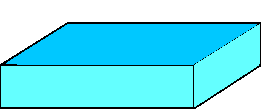
\includegraphics[width=0.25\linewidth]{../Common/images/Cell30.pdf} 
	\end{center}
	
	\item $cell_{3,1}$ : Touching one other cell. Three cells in Figure \ref{fig_cellular}a are of this type
	\begin{center}
	\includegraphics[width=0.25\linewidth]{../Common/images/Cell31.pdf} 
	\end{center}
	
	\item $cell_{3,2a}$ : Touching two other cells, but the touching faces are 'adjacent' to each other.
	\begin{center}
	\includegraphics[width=0.25\linewidth]{../Common/images/Cell32a.pdf} 
	\end{center}
	
	\item $cell_{3,2a'}$ : Touching two other cells, but the touching faces are 'non-adjacent' or 'opposite' to each other.
	\item Similarly cells with further adjacencies can be defined.
	\end{itemize}
	
	\item $cell_{2,*}$ : 2D cells (Figure \ref{fig_cellular}b), surfaces, topologically equivalent to planar surface. They are further classified similar to 3D cells, with a difference that the touching elements are edges.

\end{itemize}

\subsubsection{Steps:Topological dimension reduction}
Topological transformation of Solid (3D cells) to Surface (2D cells) happens as follows:
\begin{itemize}
[noitemsep,topsep=2pt,parsep=2pt,partopsep=2pt,leftmargin=*]
\item $cell_{i,0|1}$ transforms into $cell_{i-1,0|1}$ \label{rule_c32}
	\begin{center}
	\includegraphics[width=0.6\linewidth]{../Common/images/Cell3201.pdf} 
	\end{center}
\item $cell_{i,na'}$ transforms into $cell_{i-1,na'}$ , where $n$ is the number of non-adjacent interfaces.

\item  Adjacent types transform into just one $cell_{1,*}$ (edge) called the {\em Radial edge}.
	\begin{center}
	\includegraphics[width=0.45\linewidth]{../Common/images/Cell31a.pdf} 
	\end{center}
	
\item  Solid ($cell_{3,na'}$), being topologically similar to simple plate (and homeomorphic to Sphere), has following topological entities: 
%\vspace{-3mm}
\begin{align*}
faces=6\\edges=12\\vertices=8\\na' = n
\end{align*}
 
It gets transformed into Midsurface ($cell_{2,na'}$) as per:
%\vspace{-3mm}
\begin{equation}
\begin{aligned}
faces=1\\
edges=4-n\\
vertices=4-2n
\end{aligned}
\label{eqn_cellularna}
\end{equation}
%	\vspace{-3mm}

\item  $cell_{3,a}$ contributes following to the Midsurface
\vspace{-3mm}
\begin{equation}
\begin{aligned}
edges = 1\\
vertices = 2
\end{aligned}
\label{eqn_cellulara}
\end{equation}

\vspace{-3mm}

\end{itemize}
%\includegraphics[width=0.4\linewidth]{../Common/images/YwithHole.pdf} 
\subsubsection{Examples}
\begin{itemize}
[noitemsep,topsep=2pt,parsep=2pt,partopsep=2pt,leftmargin=*]

\item Simple plate =  $cell_{3,0}$
	\begin{itemize}
	[noitemsep,topsep=2pt,parsep=2pt,partopsep=2pt,leftmargin=*]
	\item As per equation (\ref{eqn_cellularna}) , with $n=0$, Midsurface is predicted to have 
	\begin{align*}
	faces=1\\edges=4-0\\vertices=4- 2\times0
	\end{align*}

	\item Entities match with that of Midsurface ($cell_{2,0}$) 
		\begin{align*}
		faces=1\\edges=4\\vertices=4
		\end{align*}
	 
	\end{itemize}

\item 'L' shaped part =  $2 \times cell_{3,1} + cell_{3,2a}$. 

\begin{itemize}
[noitemsep,topsep=2pt,parsep=2pt,partopsep=2pt,leftmargin=*]

\item As per equation (\ref{eqn_cellularna}) , with $n=1$, each of the two sides ($cell_{3,1}$) of the Midsurface is predicted to have  
	\begin{align*}
	faces=1\\edges=4-1\\vertices=4-2\times 1
	\end{align*}
\item As per equation (\ref{eqn_cellulara}), the common intersection ($cell_{3,2a}$) is predicted to have 
	\begin{align*}
	edges=1\\vertices=2
	\end{align*}

\item Total is 
	\begin{align*}
	faces=2\times1\\edges=2\times(4-1) + 1\\ vertices=2\times(4-2) + 2
	\end{align*}

	\item The predicted entities match with that of the actual Midsurface ($2\times cell_{2,1} +cell_{1,2}$) 
		\begin{align*}
		faces=2\\edges=7\\vertices=6
		\end{align*}
\end{itemize}


\item 'T' shaped part =  $3 \times cell_{3,1} + cell_{3,3a}$. 

\begin{itemize}
[noitemsep,topsep=2pt,parsep=2pt,partopsep=2pt,leftmargin=*]

\item As per equation (\ref{eqn_cellularna}) , with $n=1$, each of the three sides ($cell_{3,1}$) of the Midsurface is predicted to have  
	\begin{align*}
	faces=1\\edges=4-1\\vertices=4-2\times 1
	\end{align*}
\item As per equation (\ref{eqn_cellulara}), the common intersection ($cell_{3,3a}$) is predicted to have 
	\begin{align*}
	edges=1\\vertices=2
	\end{align*}

\item Total is 
	\begin{align*}
	faces=3\times1\\edges=3\times(4-1) + 1\\ vertices=3\times(4-2) + 2
	\end{align*}

	\item The predicted entities match with that of the actual Midsurface ($3\times cell_{2,1} +cell_{1,3}$) 
		\begin{align*}
		faces=3\\edges=10\\vertices=8
		\end{align*}
\end{itemize}

\item 'Hole' in Solid is a special case, 
		\begin{align*}
		genus=1\\faces=1\\edges=2\\vertices=2
		\end{align*}
		which gets converted to a hole in the surface
			\begin{align*}
	edges=1\\vertices=1
	\end{align*}

\end{itemize}

With the use of cellular decomposition of a thin solid, topological entities for its non-manifold Midsurface are predicted, which when substituted in the non-manifold equation prove the validity.

%
%In the Thin wall manifold solid faces are classified as as $f_p$ (Principal-Main faces) and $f_t$ (Thickness or capping faces). Edges are classified as $e_p$ (Principal-Main edges) and $e_t$ (along thickness or capping edges). Vertices are classified as $v_t$ (thickness vertex) when they are connected to at-least one $e_t$ and $v_p$ (principal or radial vertex), when they are connected to only $e_p$s.
%
%\subsubsection{Steps: Topological dimension reduction}
%\begin{itemize}
%[noitemsep,topsep=2pt,parsep=2pt,partopsep=2pt,leftmargin=*]
%\item Given a Manifold solid, half of the $f_p$s are retained in the corresponding Midsurface. Thickness faces $f_t$s and edges $e_t$s are gone. 
%%\item {\em Genuses} are the holes and the {\em rings} in the Midsurface
%\item Half of the thickness vertices $v_t$s will remain in the Midsurface. But the difficulty comes in predicting vertices at the junctions (corresponding to $v_p$s). Additional information about radial group of  $v_p$s is not directly available in the solid model (unless loop traversal detects cycles). 
%\item For example, in case of {\em \bf L} shape, half the $v_p$s are present in the Midsurface as radial vertices, but in case of {\em \bf T} shape thats not true. So the procedure which is valid for  junctions up to degree two, is not so for the higher degree junctions. Examples below demonstrate this.
%\item Expand the Solid equation (\ref{eqn_manifold}) to include newly defined faces, edges: $ (v_p + v_t) - (e_p  + e_t) + (f_p  + f_t) = 2 (s - g) + r$
%\item For Midsurface of this Solid, number of topological entities are changed as follows:
%	\begin{itemize}
%	[noitemsep,topsep=2pt,parsep=2pt,partopsep=2pt,label={}, leftmargin=*]
%	\item $v_{nm} = (v_p + v_t)/2$
% 	\item $e_{nm} = e_p/2$
%  	\item $e_t  = f_t  = r = 0$
%  	\item $f_{nm} = f_p/2$
%  	\end{itemize}
%\item Validate if the non-manifold equation $v_{nm} - e+{nm} + f_{nm} == (s_{nm} - g_{nm}) $ is honored.
%\end{itemize}
%
%\subsubsection{Examples}
%\begin{itemize}
%[noitemsep,topsep=2pt,parsep=2pt,partopsep=2pt,leftmargin=*]
%\item For Simple plate:
%	\begin{itemize}
%	[noitemsep,topsep=2pt,parsep=2pt,partopsep=2pt,label={}, leftmargin=*]
%%	\item \textcolor{blue}{``picture of the plate''}
%	\item $f_p =2,f_t=4,e_p=8,e_t=4,v_t=8,v_p=0,s=1,g=0$
% 	\item $v_{nm} = (v_t + v_p)/2 = 8 /2 = 4$
%  	\item $e_{nm} = e_p/2 = 8/2 = 4$
%  	\item $f_{nm} = f_p/2 = 2/2 = 1$
%  	\item $s_{nm} = 1, g_{nm} = 0$
%  	\item $v_{nm} - e_{nm} + f_{nm} = 4 - 4 +1 = 1 = (s_{nm} - g_{nm})$.
%  	\item \textbf{Result}: \textcolor{green}{Valid}
%  	\end{itemize}
%
%\item For 'L' shaped plate:
%	\begin{itemize}
%	[noitemsep,topsep=2pt,parsep=2pt,partopsep=2pt,label={}, leftmargin=*]
%%	\item \textcolor{blue}{``picture of L''}
%	\item $f_p =4,f_t=4,e_p=14,e_t=4,v_t=8,v_p=4,s=1,g=0$
% 	\item $v_{nm} = (v_t + v_p)/2 = (8+4) /2 = 6$
%  	\item $e_{nm} = e_p/2 = 14/2 = 7$
%  	\item $f_{nm} = f_p/2 = 4/2 = 2$
%  	\item $s_{nm} = 1, g_{nm} = 0$
%  	\item $v_{nm} - e_{nm} + f_{nm} = 6 - 7 + 2= 1 = (s_{nm} - g_{nm})$.
%  	\item \textbf{Result}: \textcolor{green}{Valid}
%  	\end{itemize}
%  	
%  	\item For 'T' shaped plate: 
%	\begin{itemize}
%	[noitemsep,topsep=2pt,parsep=2pt,partopsep=2pt,label={}, leftmargin=*]
%%	\item \textcolor{blue}{``picture of T''}
%	\item $f_p =5,f_t=5,e_p=20,e_t=6,v_t=12,v_p=4,s=1,g=0$
% 	\item $v_{nm} = (v_t + v_p)/2 = (12+4) /2 = 8$
%  	\item $e_{nm} = e_p/2 = 20/2 = 10$
%  	\item \textcolor{red}{$f_{nm} = f_p/2 = 5/2 = 2.5$}
%  	\item $s_{nm} = 1, g_{nm} = 0$
%  	\item $v_{nm} - e_{nm} + f_{nm} = 6 - 7 + 2= 1 = (s_{nm} - g_{nm})$.
%  	\item \textbf{Result}: \textcolor{red}{Invalid}
%  	\end{itemize}
%
%\end{itemize}
%
%\textbf{Conclusion}: Manifold equation of Thin Solid cannot be simplistically converted to Non-Manifold equation of its Midsurface. Thus this direction of validation has limitations. Following section examines if the other direction of validation is possible or not.

\subsection{Validity: Midsurface to Sheet Metal Solid}
Non-manifold topology of Midsurface contains far richer (classifiable) topological information than its corresponding solid model. For example, Midsurface of 'T' shaped solid, which can be represented as Figure \ref{fig_nonmanifold} has following classified entities:

\begin{figure}[htbp]
\includegraphics[width=0.7\linewidth]{../Common/images/NonManifoldT.pdf} 
\caption{Example: Non-manifold}
\label{fig_nonmanifold}
\end{figure}

	\begin{itemize} 
	[noitemsep,topsep=2pt,parsep=2pt,partopsep=2pt,label={},leftmargin=*]\label{list_topos}
	\item Faces ($f$): Bound by two face-uses.
	
	\item Sharp Vertex ($v_s$): Connected to two edges of the same face
	\item Sharp Edge ($e_s$): Connected to two sharp vertices

	\item Radial Vertex ($v_{r}$): Connected edges of different faces
	\item Degree ($n_{r}$) at the radial edge is the number of faces attached to it 
	\item Radial Edge ($e_{r}$): Connected between two radial vertices
	\item Sharp-Radial Edge ($e_{sr}$): Between sharp and radial vertex
	\item Internal Edge ($e_i$): Part of the inner loop
	\item Internal Vertex ($v_i$):Connected to internal edge
	\item Internal Loop ($r_i$) : Characterized by internal edges and vertices

	\end{itemize}



\subsubsection{Steps: Topological dimension addition}
Sheet Metal part can be imagined to be a thickened Midsurface \cite{SHLee2001}. If we have non-manifold equation of the Midsurface, thickness operators-relations can be derived so as to transform it into manifold Sheet Metal part. The topological entities of the generated solid are calculated as per following steps: %via relations in the Table \ref{table_TopoVal}.

\begin{itemize}
[noitemsep,topsep=2pt,parsep=2pt,partopsep=2pt,leftmargin=*]

\item Face-uses become principal faces. 
\item Face-uses around a radial edge remain as connected in the solid as well. 
%Face-uses of same face will get connected via thickness faces
\item Apart from edge-use loop corresponding to face-use, two additional loops are proposed as follows:
	\begin{itemize}
	[noitemsep,topsep=2pt,parsep=2pt,partopsep=2pt,leftmargin=*]
	\item Loop around sharp edge. This gives rise to singular capping face  (Fig. \ref{fig_loops}a)
	\item Loop around sharp-radial edge. This gives rise to a combined capping face (Fig. \ref{fig_loops}b)
	\end{itemize}
	
 \begin{figure}[htbp]
\centering \includegraphics[width=0.34\linewidth]{../Common/images/NonManifoldLoopsToFaces.pdf}
\caption{Newly proposed loops}
\label{fig_loops}
 \end{figure}
 
\item Sharp vertices will create capping edges
\item Radial vertices or edges won't create any new topological entity
\end{itemize}
Topological entities in the thickened solid are predicted as follows:
\begin{itemize}
[noitemsep,topsep=2pt,parsep=2pt,partopsep=2pt,label=\textbullet,leftmargin=*]
\item Manifold-Vertices = 2 times sharp and internal vertices (one up, one below) + degree times radial vertices to take care of junctions.
\begin{equation}
v_m = 2 (v_s + v_i) + n_r v_r \label{eqn_vm}
\end{equation}
\item Manifold-Edges = 2 times sharp, sharp-radial and internal edges (offset up and down) + degree times radial edges for offsets at junctions + sharp vertices for vertical capping edges + internal vertices for vertical seam edges
\begin{equation}
e_m = 2 (e_s + e_{sr} + e_i) + n_r e_r  + v_s + v_i\label{eqn_em}
\end{equation}
\item Manifold-Faces = 2 times faces (offset up and down) + sharp edges for capping faces as per  (Fig. \ref{fig_loops}a) + sharp edges divided by degree so that just one combined face as per  (Fig. \ref{fig_loops}b) + internal edges for capping internal faces
\begin{equation}
f_m = 2f + e_s + e_{sr}/n_r + e_i \label{eqn_fm}
\end{equation}
\item Manifold-Rings = 2 times internal rings
\begin{equation}
r_m = 2r_i\label{eqn_rm}
\end{equation}
\item Manifold-Genus = internal ring as it becomes a hole
\begin{equation}
h_m = r_i\label{eqn_hm}
\end{equation}

\end{itemize}
%
%\begin{table}
%\caption{Solid by thickening Midsurface Entities}
%\begin{tabular}[h]{@{} p{0.15\linewidth}  p{0.25\linewidth}  p{0.5\linewidth}@{}} \toprule
%{\bf Solid } & {\bf Midsurface }  & {\bf Explanation} \\
%\midrule
%%------------------------------------------------------------------------------------------------------------------------------------
%Faces ($f_m$) &
%$2f+e_s+e_{sr}/n_{r} +e_i $ &
%Double faces to make Main faces + Thickness faces + Common faces for Loop with Radial in it + inner hole face \\
%%------------------------------------------------------------------------------------------------------------------------------------
%Edges ($e_m$) &
%$2(e_s+e_{sr}+e_i )+n_{r} e_{r}+v_s+v_i  $ &
%Double (sharp + sharp-radial + internal) to represented offseted edges + $n$ edges radially offseted from $e_r$ + thickness edges one per sharp vertex + seam edge + internals\\
%%------------------------------------------------------------------------------------------------------------------------------------
%Vertices ($v_m$) &
%$2v_s+n_{r} v_r+2v_i$ &
%Double offseted vertices + $n$ times offsetting at each $v_r$+ double the offseted seam vertices\\
%%------------------------------------------------------------------------------------------------------------------------------------
%Shell ($s_m$) &
%$s$ &
%Same\\
%%------------------------------------------------------------------------------------------------------------------------------------
%Rings ($r_m$) &
%$2r_i $& 
%Double for offsetting. Assuming Sheet Metal generated only through hole and not the blind hole.\\
%%------------------------------------------------------------------------------------------------------------------------------------
%Genus  ($h_m$) &
%$r_i $&
%Through holes == genus\\
%%------------------------------------------------------------------------------------------------------------------------------------
%
%\bottomrule
%\end{tabular}
%\label{table_TopoVal}
%\end{table}

\subsubsection{Sheet Metal Midsurface Characteristic}
The predicted manifold entities (Equations \ref{eqn_vm}, \ref{eqn_em}, \ref{eqn_fm}, \ref{eqn_rm}, \ref{eqn_hm}) if honor the manifold eqution (Eqn. \ref{eqn_manifold}), then the Midsurface can be treated as a valid representation of the Sheet Metal part. 

%\vspace{-3mm}
\begin{equation}
v_m-e_m+f_m=2(s_m-h_m )+r_m
\label{eqn_manifold}
\end{equation}

Substitute for each manifold entities to get:
%\begin{itemize}
%[noitemsep,topsep=2pt,parsep=2pt,partopsep=2pt,label={}]
%\item $v_m = 2v_s+n_{r} v_r+2v_i $
%\item $e_m = 2(e_s+e_{sr}+e_i )+n_{r} e_{r}+v_s+v_i $
%\item $f_m = 2f+e_s+e_{sr}/n_{r} +e_i $
%\item $r_m = 2r_i, h_m = r_i$ ({\em genus} is half the loops)
%\end{itemize}

\vspace{-5mm}
\begin{multline}
[2 (v_s + v_i) +n_{r} v_r ]\\
-[2(e_s+e_{sr}+e_i )+n_{r} e_{r}+v_s+v_i ]\\
+[2f+e_s+e_{sr}/n_{r} +e_i ]\\
=2(s-r_i )+2r_i
\label{eqn_midsurf}
\end{multline}

Midsurface entities should also honor the Non-manifold equation (\ref{eqn_nonmanifold}):
%\vspace{-2mm}
\begin{equation}
v-e+f=1(s-h)+r
\label{eqn_nonmanifold}
\end{equation}

Expanding it with classified entities as below:
% \vspace{-3mm}
\begin{align}
[v_s+v_r+v_i]-[e_s+e_r+e_{sr}+e_i ]+[f]\\=1(s-r_i )+r_i
\label{eqn_nonmanifoldexpanded}
\end{align}

(Equation \ref{eqn_midsurf}) - 2 $\times$ (Equation  \ref{eqn_nonmanifoldexpanded}) gives
%\vspace{-3mm}
\begin{align}
v_s+(2-n_{r} ) v_{r}+v_i \\= e_s+e_i+(2-n_{r}) e_{r}+e_{sr}/n_{r}\\=\chi_{smm}
\label{eqn_nonmanifolddiff}
\end{align}

This is the new Sheet Metal Midsurface Characteristic  $\chi_{smm}$. It is just in terms of $edges$ and $vertices$. One has to check only this equation on Midsurface entities and then it is sure that the corresponding solid manifold (computed by thickening) will be valid as well.

\subsubsection{Usefulness of $\chi_{smm}$}
Following are the ways in which some of the Midsurface errors can be detected using $\chi_{smm}$
\begin{itemize}
[noitemsep,topsep=2pt,parsep=2pt,partopsep=2pt,leftmargin=*]
\item \textbf{Missing Surfaces}: Missing surface would result in less number of edges and vertices
\item \textbf{Missing Connections}: Gaps would result in less radial edges and vertices 
\end{itemize}

\subsubsection{Procedure to validate Midsurface using  $\chi_{smm}$}
\begin{enumerate}
\item Count topological entities of the Midsurface as per classification suggested in the list (\ref{list_topos}) .
\item Predict topological entities of the corresponding thin-wall solid using equations ( \ref{eqn_vm}, \ref{eqn_em}, \ref{eqn_fm}, \ref{eqn_rm}, \ref{eqn_hm}).
\item Verify that the topological entities of the Midsurface satisfy the non-manifold equation (Equation \ref{eqn_nonmanifold}), by showing that left ($\chi_{nm-left}$) and right  ($\chi_{nm-right}$) hand side of the equation matches.
\item Verify that the predicted topological entities of the  thin-wall solid satisfy the manifold equation (Equation \ref{eqn_manifold}), by showing that left ($\chi_{m-left}$) and right  ($\chi_{m-right}$) hand side of the equation matches. Thus proving that the transformation equations used to predict, are valid. Same validity can be shown using just the $\chi_{smm}$ characteristic, as below.
\item Verify that  $\chi_{smm}$ characteristic equation (Equation \ref{eqn_nonmanifolddiff}) matches. 
\end{enumerate}



\subsubsection{Examples}
Following examples show the validation of Midsurface using newly proposed $\chi_{smm}$ Characteristic:

\vspace{2mm}

\begin{enumerate}
[noitemsep,topsep=2pt,parsep=2pt,partopsep=2pt,leftmargin=*]
\item Simple Plate %(Table \ref{table_TopoValPlate})

%\vspace{3mm}
\begin{center}
\includegraphics[width=0.35\linewidth]{../Common/images/SimplePlate.pdf} 
\end{center}
%\vspace{3mm}

\begin{enumerate}
%[noitemsep,topsep=2pt,parsep=2pt,partopsep=2pt,label=\textbullet,leftmargin=*]
\item Midsurface entities: \\$f = 1, e_s = 4, e_{sr} = 0, e_r = 0, e_i=0,$\\$v_s = 4,v_r =0, v_i= 0, s=1,h=0,r=1$
\item Predicted solid-faces: \\$f_m = 2f+e_s+e_{sr}/n_{r} +e_i $\\$= 2+4+0+0 = 6$
\item Predicted solid-edges: \\ $e_m = 2(e_s+e_{sr}+e_i )+n_{r} e_{r}+v_s+v_i $\\$= 2(4+0+0)+0+4+0 = 12$
\item Predicted solid-vertices: \\$v_m = 2v_s+n_{r} v_r+2v_i$\\$=2\times4 + 0 + 0=8$
\item Predicted solid-shells-holes: \\$s_m =s = 1, h_m = r_i  = 0, r_m = 2r_i = 0$
\item Non-manifold equation left side  $\chi_{nm-left} $\\$= v-e+f $\\$= 4-4+1 = 1$
\item Non-manifold equation right side  $\chi_{nm-right}$\\$=s-h+r$\\$=1-0+0 = 1$
\item Manifold equation left side  $\chi_{m-left} $\\$= v_m-e_m+f_m $\\$=8-12+6= 2$
\item Manifold equation right side  $\chi_{m-right}$\\$=2(s_m-h_m )+r_m$\\$= 2(1-0)+0 = 2$
\item Sheet Metal Midsurface Characteristic $\chi_{smm}$\\$=
e_s+e_i+(2-n_{r} ) e_{r}+e_{sr}/n_{r} $\\$=v_s+(2-n_{r} ) v_{r}+v_i$\\$ 4+0+0+0=4+0+0= 4$
\item \textbf{Result}: \textcolor{green}{Matches}
\end{enumerate}
%%----------------------------------------------------------------------------------------
%\begin{table}
%\caption{Simple Plate}
%\begin{tabular}[t]{@{} p{0.035\linewidth}  p{0.035\linewidth} |  p{0.035\linewidth}  p{0.47\linewidth}  p{0.23\linewidth}@{}} \toprule
%{\bf NM } & {\bf \# }  & {\bf M} & {\bf Conversion } & {\bf Solid \# }  \\
%\midrule
%
%$f$ &
%$1$ &
%$f_m$ &
%$2f+e_s+e_{sr}/n_{r} +e_i $ &
%$2+4+0+0 = 6$\\
%
%$e_s$ &
%$4$ &
%$e_m$&
%$2(e_s+e_{sr}+e_i )+n_{r} e_{r}+v_s+v_i $&
%$2(4+0+0)+0+4+0 = 12$\\
%
%$e_{sr}$&
%$0$&
%$v_m$&
%$2v_s+n_{r} v_r+2v_i $&
%$2\times4 + 0 + 0=8$\\
%
%$e_r$&
%$0$&
%$s_m$&
%$s $&
%$1$\\
%
%$e_i$&
%$0$&
%$h_m$&
%$r_i $&
%$0$\\
%
%$v_s$&
%$4$&
%$r_m$&
%$2r_i $&
%$0$\\
%
%$v_r$&
%$0$&
%&
%NM Characteristic left side  $\chi_{nm-left}$ &
%$4-4+1 = 1$\\
%
%$v_i$&
%$0$&
%&
%NM Characteristic right side  $\chi_{nm-right}$ &
%$1-0+0 = 1$\\
%
%$s$&
%$1$&
%&
%M Characteristic left side  $\chi_{m-left}$ &
%$8+6-12 = 2$\\
%
%$h$&
%$0$&
%&
%M Characteristic right side  $\chi_{m-right}$ &
%$2(1-0)+0 = 2$\\
%
%$r$&
%$1$&
%&
%Sheet Metal Midsurfaces Characteristic $\chi_{smm}$ ,
%$e_s+e_i+(2-n_{r} ) e_{r}+e_{sr}/n_{r} =v_s+(2-n_{r} ) v_{r}+v_i $ &
%$4+0+0+0=4+0+0= 4$\\
%\bottomrule
%\end{tabular}
%\label{table_TopoValPlate}
%\end{table}
%%----------------------------------------------------------------------------------------

\item Y with hole on one leg% (Table \ref{table_TopoValY})

%\vspace{3mm}
\begin{center}
\includegraphics[width=0.3\linewidth]{../Common/images/YwithHole.pdf} 
\end{center}
%\vspace{3mm}

\begin{enumerate}
%[noitemsep,topsep=2pt,parsep=2pt,partopsep=2pt,label=\textbullet,leftmargin=*]
\item Midsurface entities: \\ $f = 3, e_s = 3, e_{sr} = 6, e_r = 1, e_i=1,v_s = 6,v_r =2, v_i= 1, s=1,h=0,r=1$
\item Predicted solid-faces: \\ $f_m = 2f+e_s+e_{sr}/n_{r} +e_i  $\\$= 6+3+2+1=12$
\item Predicted solid-edges: \\$e_m = 2(e_s+e_{sr}+e_i )+n_{r} e_{r}+v_s+v_i $\\$= 2(3+6+1)+3+6+1 =30$
\item Predicted solid-vertices:  $v_m = 2v_s+n_{r} v_r+2v_i $\\$=2\times6+ 6 + 2=20$
\item Predicted solid-shells-holes: $s_m =s = 1,h_m = r_i  = 1, r_m = 2r_i = 2$
\item Non-manifold equation left side  $\chi_{nm-left}$\\$= v-e+f $\\$= 9-11+3=1$
\item Non-manifold equation right side  $\chi_{nm-right}$\\$=s-h+r$\\$=1-1+1 = 1$
\item Manifold equation left side  $\chi_{m-left}$\\$= v_m-e_m+f_m$\\$=20-30+12 = 2$
\item Manifold equation right side  $\chi_{m-right} $\\$=2(s_m-h_m )+r_m$\\$= 2(1-1)+2 = 2$
\item Sheet Metal Midsurface Characteristic $\chi_{smm}$ \\$=
e_s+e_i+(2-n_{r} ) e_{r}+e_{sr}/n_{r} $\\$=v_s+(2-n_{r} ) v_{r}+v_i$\\$ 3+1+(2-3)+2=6+(2-3)2+1=5$
\item \textbf{Result}: \textcolor{green}{Matches}
\end{enumerate}

%----------------------------------------------------------------------------------------
%\begin{table}
%\caption{Y with a hole on one leg}
%\begin{tabular}[t]{@{} p{0.035\linewidth}  p{0.035\linewidth} |  p{0.035\linewidth}  p{0.47\linewidth}  p{0.23\linewidth}@{}} \toprule
%{\bf NM } & {\bf \# }  & {\bf M} & {\bf Conversion } & {\bf Solid \# }  \\
%\midrule
%
%$f$ &
%$3$ &
%$f_m$ &
%$2f+e_s+e_{sr}/n_{r} +e_i $ &
%$12$\\
%
%$e_s$ &
%$3$ &
%$e_m$&
%$2(e_s+e_{sr}+e_i )+n_{r} e_{r}+v_s+v_i $&
%$30$\\
%
%$e_{sr}$&
%$6$&
%$v_m$&
%$2v_s+n_{r} v_r+2v_i $&
%$20$\\
%
%$e_r$&
%$1$&
%$s_m$&
%$s $&
%$1$\\
%
%$e_i$&
%$1$&
%$h_m$&
%$r_i $&
%$1$\\
%
%$v_s$&
%$6$&
%$r_m$&
%$2r_i $&
%$2$\\
%
%$v_r$&
%$2$&
%&
%NM Characteristic left side  $\chi_{nm-left}$ &
%$9-11+3 = 1$\\
%
%$v_i$&
%$1$&
%&
%NM Characteristic right side  $\chi_{nm-right}$ &
%$1-1+1 = 1$\\
%
%$s$&
%$1$&
%&
%M Characteristic left side  $\chi_{m-left}$ &
%$20-30+12 = 2$\\
%
%$h$&
%$1$&
%&
%M Characteristic right side  $\chi_{m-right}$ &
%$2(1-1)+2 = 2$\\
%
%$r$&
%$1$&
%&
%Sheet Metal Midsurfaces Characteristic $\chi_{smm}$,
%$e_s+e_i+(2-n_{r} ) e_{r}+e_{sr}/n_{r} =v_s+(2-n_{r} ) v_{r}+v_i $ &
%
%$3 + 1 + (2-3) + 2 = 6 + (2 -3)2 + 1 = 5$\\
%\bottomrule
%\end{tabular}
%\label{table_TopoValY}
%\end{table}
%----------------------------------------------------------------------------------------
%\item Closed Box of Surfaces  (Table \ref{table_TopoValClosedBox})
%
%\vspace{2mm}
%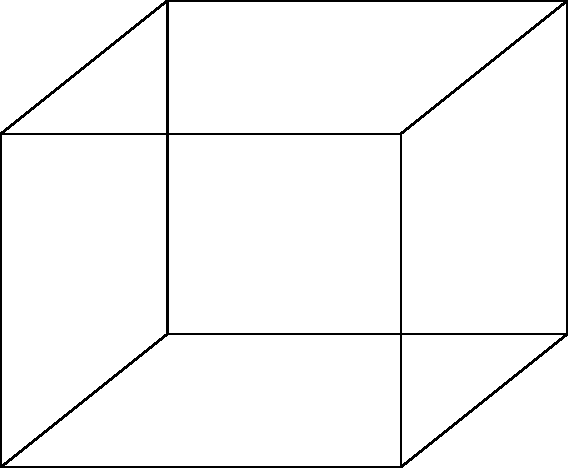
\includegraphics[width=0.6\linewidth]{../Common/images/ClosedBox.pdf} 
%\vspace{2mm}
%
%%----------------------------------------------------------------------------------------
%\begin{table}
%\caption{Closed Box of Surfaces}
%\begin{tabular}[t]{@{} p{0.035\linewidth}  p{0.035\linewidth} |  p{0.035\linewidth}  p{0.47\linewidth}  p{0.23\linewidth}@{}} \toprule
%{\bf NM } & {\bf \# }  & {\bf M} & {\bf Conversion } & {\bf Solid \# }  \\
%\midrule
%
%$f$ &
%$6$ &
%$f_m$ &
%$2f+e_s+e_{sr}/n_{r} +e_i $ &
%$12$\\
%
%$e_s$ &
%$0$ &
%$e_m$&
%$2(e_s+e_{sr}+e_i )+n_{r} e_{r}+v_s+v_i $&
%$24$\\
%
%$e_{sr}$&
%$0$&
%$v_m$&
%$2v_s+n_{r} v_r+2v_i $&
%$16$\\
%
%$e_r$&
%$12$&
%$s_m$&
%$s $&
%$2$\\
%
%$e_i$&
%$0$&
%$h_m$&
%$r_i $&
%$0$\\
%
%$v_s$&
%$0$&
%$r_m$&
%$2r_i $&
%$0$\\
%
%$v_r$&
%$8$&
%&
%NM Characteristic left side  $\chi_{nm-left}$ &
%$8-12+6=2$\\
%
%$v_i$&
%$0$&
%&
%NM Characteristic right side  $\chi_{nm-right}$ &
%$2-0+0=2$\\
%
%$s$&
%$2$&
%&
%M Characteristic left side  $\chi_{nm-left}$ &
%$16-24+12=4$\\
%
%$h$&
%$0$&
%&
%M Characteristic right side  $\chi_{nm-right}$ &
%$4$\\
%
%$r$&
%$0$&
%&
%Sheet Metal Midsurfaces Characteristic $\chi_{smm}$,
%$e_s+e_i+(2-n_{r} ) e_{r}+e_{sr}/n_{r} =v_s+(2-n_{r} ) v_{r}+v_i $ &
%
%$0$\\
%\bottomrule
%\end{tabular}
%\label{table_TopoValClosedBox}
%\end{table}
%----------------------------------------------------------------------------------------
\end{enumerate}

